\begin{frame}
  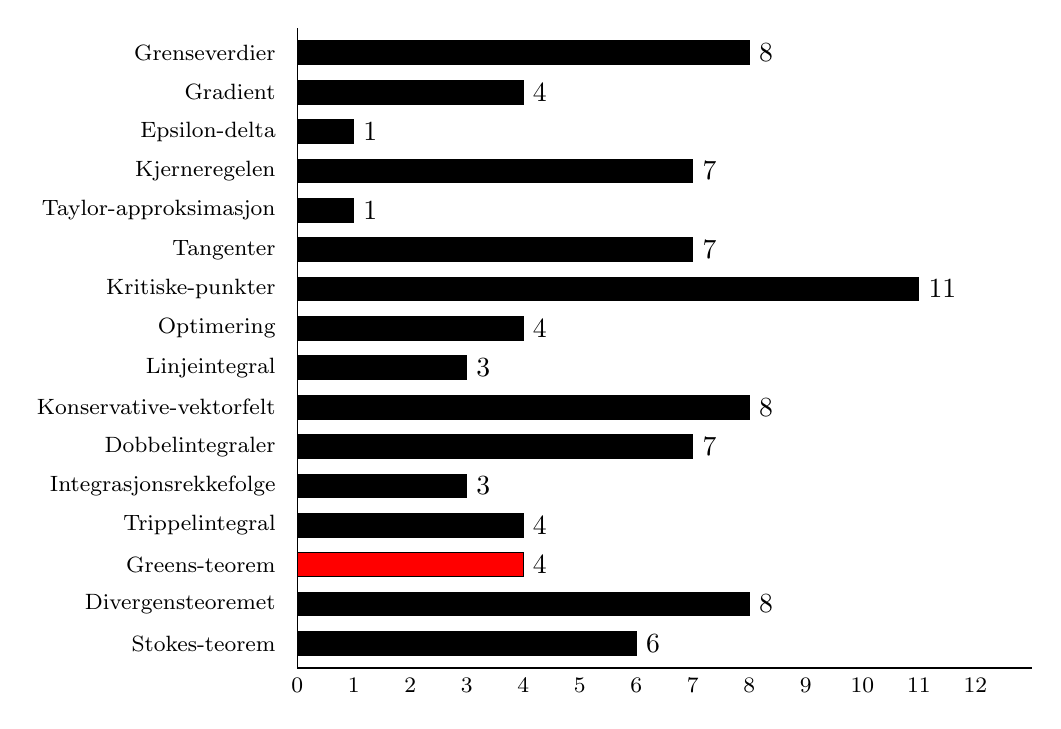
\begin{tikzpicture}
    \begin{axis}[ xbar=0pt, /pgf/bar shift=0pt, legend style={ legend columns=4,
        at={(xticklabel cs:0.5)}, anchor=north, draw=none }, ytick={0,...,15},
      ytick style={draw=none},% <- added
      axis y line*=none, axis x line*=bottom, tick label
      style={font=\footnotesize}, legend style={font=\footnotesize}, label
      style={font=\footnotesize}, xtick style={draw=none},% <- added
      xtick={0,1,...,12}, width=.9\textwidth, bar width=3mm, y dir = reverse,
      xmin=0, xmax=13, area legend,
      y=5mm, enlarge y limits={abs=0.625},
      style={text=black}, every axis plot/.append style={fill},
      nodes near coords, nodes near coords,
      yticklabels={%
        {\topicref{Grenseverdier}},
        {\topicref{Gradient}},
        {\topicref{Epsilon-delta}},
        {\topicref{Kjerneregelen}},
        {\topicref{Taylor-approksimasjon}},
        {\topicref{Tangenter}},
        {\topicref{Kritiske-punkter}},
        {\topicref{Optimering}},
        {\topicref{Linjeintegral}},
        {\topicref{Konservative-vektorfelt}},
        {\topicref{Dobbelintegraler}},
        {\topicref{Integrasjonsrekkefolge}},
        {\topicref{Trippelintegral}},
        {\topicref{Greens-teorem}},
        {\topicref{Divergensteoremet}},
        {\topicref{Stokes-teorem}}}]
      \addplot[fill=black] coordinates {(8,0)};
      \addplot[fill=black] coordinates {(4,1)};
      \addplot[fill=black] coordinates {(1,2)};
      \addplot[fill=black] coordinates {(7,3)};
      \addplot[fill=black] coordinates {(1,4)};
      \addplot[fill=black] coordinates {(7,5)};
      \addplot[fill=black] coordinates {(11,6)};
      \addplot[fill=black] coordinates {(4,7)};
      \addplot[fill=black] coordinates {(3,8)};
      \addplot[fill=black] coordinates {(8,9)};
      \addplot[fill=black] coordinates {(7,10)};
      \addplot[fill=black] coordinates {(3,11)};
      \addplot[fill=black] coordinates {(4,12)};
      \addplot[fill=red] coordinates {(4,13)};
      \addplot[fill=black] coordinates {(8,14)};
      \addplot[fill=black] coordinates {(6,15)};
    \end{axis}
  \end{tikzpicture}
\end{frame}

\begin{frame}
    \subsection{Greens teorem}\label{subsec:Greens-teorem}
  \frametitle{Greens teorem}
  \begin{theorem}[Greens theorem]
    La $\partial D$ være en positivt orientert, stykkevis glatt, enkel, lukket
    kurve og la $D$ være området innelukket av $\partial D$. Dersom $\F(x,y) = F_1(x,y)\I +
    F_2(x,y)\J$ og $\F$ har kontinuerlige partiellderiverte på hele $D$ så er
    %
    \begin{equation*}
      \int_{\partial D} \F \cdot \dr
      = \int_{\partial D} F_1 \dx + F_2 \dy
      = \iint_D \left( \diffp{{F_2}}{x} - \diffp{{F_1}}{y} \right) \dd (x,y).
    \end{equation*}
  \end{theorem}
  \begin{figure}
  \centering
  \begin{minipage}{.45\textwidth}
    \centering
  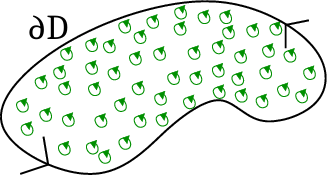
\includegraphics[width=\linewidth]{../img/greens-1.png}
\end{minipage}
\begin{minipage}{.45\textwidth}
    \centering
  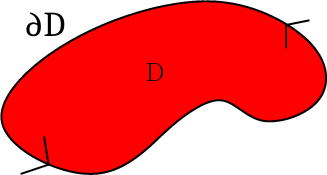
\includegraphics[width=\linewidth]{../img/greens-2.png}
\end{minipage}
\end{figure}

\end{frame}

\begin{frame}
  \frametitle{Greens teorem}
  \begin{intuisjon}
    \centering
    \begin{minipage}{.30\textwidth}
      \centering
      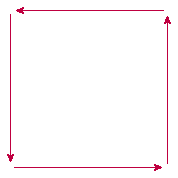
\includegraphics[width=\linewidth]{../img/Greens-intuition-1}%
    \end{minipage}\qquad
    \begin{minipage}{.30\textwidth}
      \centering
      \only<1>{\phantom{11111111111111111111}}
      \only<2>{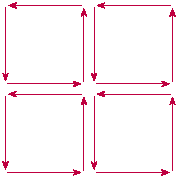
\includegraphics[width=0.95\linewidth]{../img/Greens-intuition-2}}
      \only<3->{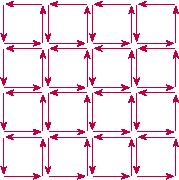
\includegraphics[width=0.95\linewidth]{../img/Greens-intuition-3}}
    \end{minipage}
    \begin{equation*}
      \only<1>{\hspace{1cm}}
      \only<4-5>{\hspace{0.25cm}}
      \only<5>{\hspace{0.5cm}}
      \int_{\partial D} \F \cdot \dr \visible<2->{ \only<2-3>{\hspace{0.5cm}}\only<4-5>{\hspace{0.25cm}}\quad = \quad \only<4-5>{\hspace{0.25cm}}\only<2-3>{\hspace{0.5cm}}\only<5>{\iint_{D} \left( \diffp{{F_2}}{x} - \diffp{{F_1}}{y} \right) \dd (x,y)}\only<4>{\iint_{D} \2d-curl \F \dd (x,y)}\only<2-3>{\int_{\partial D} \F \cdot \dr}}
      \only<1>{\phantom{\quad = \quad \iint_{D} \2d-curl \F \dd (x,y)}}
    \end{equation*}
    Med andre ord kanseleres alle de mikroskopiske sirkulasjonene slik at en
    står igjen med den makroskopiske sirkulasjonen, altså linjeintegralet.
  \end{intuisjon}
\end{frame}

\begin{frame}
  \begin{oppgave}{V2014, Oppgave , Oppgave 5} Regn ut
    $\displaystyle\int_{\partial D} \bigl(  5y - e^{\sin x} \bigr) \dx + \bigl(
    10x - \sin(y^3 + 8y) \bigr) \dy $ der $\partial D$ er en sirkel med radus $2$ og
    sentrum $(a,b)$. Spesifiser om du regner integralet med eller mot klokka.
  \end{oppgave}
  \only<1-3>{\pause
  \textbf{Steg 1:} Siden linjeintegralet vårt er på formen $\displaystyle\int_C P \dx + Q \dy$
  og vi integrerer over en lukket kurve er det logisk å tenke Greens.

  \pause
  \textbf{Steg 2:} Sjekker om vilkårene for å bruke Greens er oppfylt:
  \begin{itemize}
    \item Kurven $\partial D$ er lukket, glatt og enkel.
    \item Da alle polynomer, eksponensialfunksjoner og sinus/cosinus er deriverbare, har $\F$ kontinuerlige
      partiellderiverte.
  \end{itemize}
  \textbf{Merk:} For at for å bruke Green's må $\partial D$ orienteres
  \emph{mot-klokken}.}

  \visible<4->{
  \textbf{Steg 3:} Bruk Green's til å beregn linjeintegralet
  \begin{align*}
    I = & \iint_{\partial D} \bigl(  5y - e^{\sin x} \bigr) \dx + \bigl(
          10x - \sin(y^3 + 8y) \bigr) \dy \\
    \overset{\text{Greens teorem}}{=} & \iint_{D} \left( \diffp{}{x}\left( 10x - \sin(y^3 + 8y) \right) - \diffp{}{y}\left( 5y - e^{\sin x} \right)\right) \dd(x,y) \\
    \only<5->{= & \iint_{D} \left( \diffp{}{x}\left( 10x - 0 \right) - \diffp{}{y}\left( 5y - 0 \right)\right) \dd(x,y)} \\
    \only<6>{= & \iint_{D} ( 10 - 5) \dd(x,y)\\}
    \only<7->{=& 5 \iint_{D} \dd(x,y) }
    \only<8->{ = 5 \text{Areal}(D) }
    \only<9->{  = 5 (\pi \cdot 2^2) = 20 \pi}
  \end{align*}}
\end{frame}


%%% Local Variables:
%%% mode: latex
%%% TeX-master: "main"
%%% End:
